% Use only LaTeX2e, calling the article.cls class and 12-point type.

\documentclass[12pt]{article}

% My packages

\usepackage{graphicx}
\usepackage{amsthm}
\newtheorem{mydef}{Definition}
\usepackage{dcolumn}
\usepackage{multirow}
\usepackage{booktabs}
\newcolumntype{d}{D{.}{.}{4.0}}
\newcolumntype{s}{D{.}{.}{1.4}}

% Users of the {thebibliography} environment or BibTeX should use the
% scicite.sty package, downloadable from *Science* at
% www.sciencemag.org/about/authors/prep/TeX_help/ .
% This package should properly format in-text
% reference calls and reference-list numbers.

\usepackage{scicite}

% Use times if you have the font installed; otherwise, comment out the
% following line.

\usepackage{times}

% The preamble here sets up a lot of new/revised commands and
% environments.  It's annoying, but please do *not* try to strip these
% out into a separate .sty file (which could lead to the loss of some
% information when we convert the file to other formats).  Instead, keep
% them in the preamble of your main LaTeX source file.


% The following parameters seem to provide a reasonable page setup.

\topmargin 0.0cm
\oddsidemargin 0.2cm
\textwidth 16cm 
\textheight 21cm
\footskip 1.0cm


%The next command sets up an environment for the abstract to your paper.

\newenvironment{sciabstract}{%
\begin{quote} \bf}
{\end{quote}}


% If your reference list includes text notes as well as references,
% include the following line; otherwise, comment it out.

\renewcommand\refname{References and Notes}

% The following lines set up an environment for the last note in the
% reference list, which commonly includes acknowledgments of funding,
% help, etc.  It's intended for users of BibTeX or the {thebibliography}
% environment.  Users who are hand-coding their references at the end
% using a list environment such as {enumerate} can simply add another
% item at the end, and it will be numbered automatically.

\newcounter{lastnote}
\newenvironment{scilastnote}{%
\setcounter{lastnote}{\value{enumiv}}%
\addtocounter{lastnote}{+1}%
\begin{list}%
{\arabic{lastnote}.}
{\setlength{\leftmargin}{.22in}}
{\setlength{\labelsep}{.5em}}}
{\end{list}}


% Include your paper's title here

\title{Computational hysteresis:\\ inter-task effects in human computation} 


% Place the author information here.  Please hand-code the contact
% information and notecalls; do *not* use \footnote commands.  Let the
% author contact information appear immediately below the author names
% as shown.  We would also prefer that you don't change the type-size
% settings shown here.

\author
{Edward Newell, Derek Ruths,\\
\\
\normalsize{\texttt{edward.newell@mail.mcgill.ca}}\\
\normalsize{\texttt{druths@networkdynamics.org}}\\
\normalsize{School of computer science, McGill University,}\\
\normalsize{3630 rue University, Montreal, Quebec, H3A 0C6, Canada}\\
\\
}

% Include the date command, but leave its argument blank.

\date{}



%%%%%%%%%%%%%%%%% END OF PREAMBLE %%%%%%%%%%%%%%%%



\begin{document} 

% Double-space the manuscript.

\baselineskip24pt

% Make the title.

\maketitle 



% Place your abstract within the special {sciabstract} environment.

\begin{sciabstract}
Microtask platforms offer a fast, flexble, and inexpensive source of labour for
clerical tasks \cite{Finnerty2013, chandler2013breaking, Berinsky2012351} and 
recently have been adopted by researchers to augment datasets and solicit 
participants \cite{paolacci2010running, Berinsky2012351, chandler2013breaking}.
Computer scientists have described such platforms as a new computing 
architecture, and seek to characterize “human co-processing units” (HPUs) in 
analogy to CPUs and GPUs \cite{5543192}. However, it is known that people are 
susceptible to 
priming effects\cite{No2007,Swaab200299,Gopher2000308,sohn2001task,Ghuman17062008,BJOP1796,BJOP1826,Gass1999549}, which stands to complicate the HPU 
perspective.  Here, we introduce a framework to recast this psychological 
phenomenon as a kind of computational hysteresis. 
We apply this framework to study \textit{inter-task effects} that arise when 
microtask 
workers perform a sequence of tasks. Surprisingly, earlier tasks can have a 
very strong influence on workers during later tasks---stronger than overtly
framing the tasks as serving different research goals.   
This result has major implications for the design of crowdsourcing initiatives.
The framework we introduce provides a general measure of priming severity, 
and, in combination with machine learning tools, enables measurement without
knowing ahead of time how priming will affect output.
\end{sciabstract}

\section*{Introduction}
Microtask crowdsourcing platforms like Amazon Mechanical Turk (MTurk) make it 
possible for requesters to submit batches of small tasks to a large pool of 
workers, who do the tasks for fun, a sense of purpose, and remuneration 
\cite{kazai2013analysis,Antin20122925}.  
Originally used to distribute clerical work, these platforms 
increasingly serve as a means to engage experimental 
participants in a research 
setting \cite{paolacci2010running,Berinsky2012351,snow2008cheap,alonso2009can}.
Typical tasks include tagging and categorizing images 
\cite{6116320,Zhai2012357}, transcribing voice recordings 
\cite{chandler2013breaking,paolacci2010running}
or handwritten notes \cite{Berinsky2012351,Finnerty2013}, and judging the 
relevancy of search results \cite{le2010ensuring,grady2010crowdsourcing,alonso2009can,kazai2013analysis}

The task requester can interact with the platform like a compute server, 
seamlessly 
integrating human and machine computation.  Researchers coined the 
term HPU (Human co-Processing Unit), viewing the introduction 
of microtask platforms as a new computing architecture\cite{5543192}.  
Attempts have been made to formalize the HPU instruction set, and libraries 
that provide high-level APIs (Application Programming Interfaces) for writing 
algorithms involving human computation have been developed \cite{little2010turkit,minder2011crowdlang,minder2012crowdlang,kittur2011crowdforge}.

Here, we highlight an important way in which HPUs differ from CPUs, with 
serious implications for any crowdsourcing initiative.  Common sense would 
dictate that people's output during a task will be stochastic: when the same
task is given to different people, or given to the same person at different 
times,
the outputs may, in general, differ.  Stochasticity is not itself problematic,
since the analysis of probabilistic algorithms is fairly 
well-understood. But other non-random effects may also bear on HPU output. 
It is known that people are susceptible to priming effects 
\cite{BJOP1796,No2007,beller1971priming}, and, in particular, task-repetition 
effects \cite{Gass1999549,sohn2001task}.  

Such repetition effects, or
\textit{inter-task effects}, are neither random, nor are they formally part 
of the instructions given to the HPU.  The ``leakage'' of information, 
from recently performed tasks, into HPU outputs, is a potentially strong 
source of systematic bias.
Inter-task effects would amount to a kind of \textit{hysteresis}, meaning 
that HPU output is not only a function of the current input, but also of the 
history of inputs.  

Here we make two contributions towards understanding inter-task effects,
and HPU hysteresis in general.  We present a framework for treating this 
source of bias in the context of HPU algorithms, and we measure the impact of
inter-task effects experimentally.

Using the  Amazon Mechanical Turk (Mturk) platform, we solicited workers to 
perform a series of image-labeling tasks.  We chose this as the canonical
microtask because image labeling tasks are one of the most common kinds of
microtasks
\cite{chandler2013breaking,Berinsky2012351,Finnerty2013,paolacci2010running}, 
and it seems likely that human computation will have a long-term role
in computer vision research \cite{5543192}.
In these tasks, workers labeled images featuring iconic cultural scenes,
food, table-settings, and various utensils and cookware. We divided the set of 
images shown to a given worker into an \textit{initial} and \textit{test} set, 
but, crucially, there was no apparent distinction between these sets from the
perspective of the worker.  We varied the initial set of images, while 
keeping the test set the same, to analyze the effect that that the initial 
images had on the labels that workers attributed to the test set.

There has been considerable investigation into the factors that affect the 
quality and nature of microtask work.  These include such factors as the 
level of 
pay \cite{kazai2013analysis}, training \cite{le2010ensuring}, pre-screening of 
workers \cite{paolacci2010running}, and user-interface design 
\cite{Finnerty2013}.  Researchers have also investigated \textit{framing}, 
by testing the effects of describing the workflow context 
\cite{Kinnaird2012281}, the purpose of tasks 
\cite{chandler2013breaking}, or using an alternative problem discription
\cite{thibodeau2013natural}.  To our knowledge, no study has investigated 
inter-task effects on microtask platforms.

As a point of comparison, we included treatments in which we induce 
\textit{framing}.
Before the workers label images, we indicate that the work 
was funded by a research lab having a particular area of interest, to see the 
influence this has on the workers’ subsequent labels. 
Surprisingly, inter-task effects were stronger than framing, in some cases 
about twice as strong. 
Our results suggest that initial tasks can change what workers choose to focus
in in later tasks.  We also found that inter-task 
effects altered the level of specificity of worker's labels.  This suggests 
that careful consideration should be given to the bundling of 
tasks when designing a study using a microtask platform.

To characterize inter-task effects, we present a novel, generalized definition 
of \textit{HPU priming}. Priming is traditionally used to elucidate the
internal psychological mechanisms of cognition.  But here we are concerned with
understanding the outward effects that priming phenomena have on HPU 
algorithms. Thus, before we discuss inter-task effects experimentally, we 
describe candidate definitions for priming as computational phenomenon.  This 
leads to a natural definition of priming that provides a consistent measure of 
the severity of priming accross applications, and enables the measurement of 
priming using machine learning tools.

\paragraph*{Priming as computational hysteresis.}
To begin, we adopt the perspective that there is no canonical neutral or
unprimed state.  Rather, we will speak of one HPU population being 
\textit{differently primed} from another.  We present three definitions for 
the difference in priming between HPU populations, each with different 
advantages, and then we discuss their relationships. To proceed with the 
definitions, we will assume that two populations of HPU’s, $\mathcal{P}$ and 
$\mathcal{Q}$ were 
sampled randomly from the same initial population $\mathcal{R}$, and then were 
exposed to (possibly) different priming treatments. The HPUs in $\mathcal{P}$ 
and $\mathcal{Q}$ perform some task, leading to popualtions of work-products, 
$P$ and $Q$.

For the first defenition, we focus on the effect that differently primed
HPUs can have on the output of a human computation algorithm.

\begin{mydef}
	\label{def:bias}
	{\upshape Maximum Bias $\theta_\mathrm{bias}$:}
	Let $\mathcal{D}$ be a binary decision algorithm, which takes a 
	work-product
	$r \in P \cup Q$ as input, and outputs a bit $\mathcal{D}(r)=b$, where 
	$b \in \{0,1\}$. Denote the \emph{bias} of $\mathcal{D}$, due to the
	different priming of $\mathcal{P}$ and $\mathcal{Q}$ by
	$\theta^\mathcal{D}_\mathrm{bias}(P,Q)$ and define it to be the difference 
	in the expected output of $\mathcal{D}$ when acting on work-products from 
	$P$ and $Q$:
	$$
	\theta^\mathcal{D}_\mathrm{bias}(P,Q) = 
		\left| 
			\mathrm{E}\left\{ \mathcal{D}(p) \right\} 
			- \mathrm{E}\left\{ \mathcal{D}(q) \right\} 
		\right|,
	$$
	where $p \in P$, $q \in Q$.  Then, define the difference in priming 
	between $\mathcal{P}$ and $\mathcal{Q}$ to be the worst-case bias, i.e. 
	the bias of the most susceptible decision:
	$$
	\theta_\mathrm{bias} = 
		\sup_\mathcal{D} \theta^\mathcal{D}_\mathrm{bias}(P,Q)
	$$
\end{mydef}
In \textbf{Definition \ref{def:bias}}, $\theta_\mathrm{bias}$ has the 
straightforward interpretation as an upper bound on the amount of bias induced 
on any yes-or-no decision, due to the difference in priming of 
$\mathcal{P}$ and $\mathcal{Q}$.  Though easy to interpret, it is admittedly
not clear how $\theta_\mathbf{bias}$ could be measured in practice.

Next we to phrase the difference in priming between $\mathcal{P}$ and
$\mathcal{Q}$ in terms of the extent to which their work-products are 
distinguishable algorithmically. To facilitate this definition, we make 
use of the notions of a \textit{distinguisher} and a \textit{validation test}.
\begin{mydef}
	{\upshape Algorithmic distinctness $\theta_\mathrm{dist}$:}
	Let $\mathcal{D}$ be a distinguisher algorithm, which takes work-product 
	$r \in P \cup Q$ as input, and outputs a \emph{guess} 
	$\mathcal{D}(r) \in \{0, 1\}$. Now define a validation test 
	$V(\mathcal{D}, R_0, R_1)$ as follows. A bit is drawn uniformly at random, 
	$b \in_R \{0, 1\}$, and then a work-product $r$ is chosen uniformly at 
	random from one of the populations, decided by the bit: $r \in_R R_b$. 
	Input $r$ into $\mathcal{D}$, and if $\mathcal{D}(r) = b$, we say 
	$\mathcal{D}$ \emph{guessed correctly}, and the value of $V$ is 1, 
	otherwise $V = 0$.

	A distinguisher that guesses randomly will still be correct half of the 
	time. Therefore, denote the performance of $\mathcal{D}$ by 
	$\eta_\mathcal{D}(P, Q)$, and let
	$$
		\eta_\mathcal{D}(P,Q) = 2\cdot \mathrm{E}\{V(\mathcal{D},P,Q)\} - 1.
	$$
	Then define the difference in priming between $\mathcal{P}$ and 
	$\mathcal{Q}$ to be the performance of the best possible distinguisher:
	$$ 
		\theta_\mathrm{dist} = \sup_\mathcal{D} \eta_\mathcal{D}(P,Q)
	$$
	\label{def:dist}
\end{mydef}
In \textbf{definition \ref{def:dist}}, the performance simply rescales 
accuracy, so that when
accuracy is 1/2 (i.e. no better than chance) performance is 0, and when 
accuracy is perfect, performance is 1. This definition formulates the 
measurement of 
priming effects in terms of a binary classification problem. As we will show,
this allows us to apply machine learning tools to the 
measurement of priming.  However, it is not immediately clear 
how this measure relates to the potential for priming to cause bias.

For the third definition, we focus on describing the inherent, statistical
difference between work-products in $P$ and $Q$.  
\begin{mydef}
	\label{def:l1}
	{\upshape Total variational distance $\theta_{l_1}$:}
	Define the difference in priming between $\mathcal{P}$ and $\mathcal{Q}$ 
	to be equal to the total variational distance (also known as 
	$l_1$-distance, denoted $D_{l_1}$) between the work-products $P$ and $Q$:
	$$
	\theta_{l_1} = D_{l_1}(P,Q) \equiv \frac{1}{2} \sum_{x \in \mathcal{X}} 
	\left| 
		f_P(x) - f_Q(x)
	\right|,
	$$
	where $f_P(x)$ denotes the probability of observing x when sampling from P.
\end{mydef}
The advantage of \textbf{definition \ref{def:l1}} is that it provides connections
to statistical and information theory.

Remarkably, all three definitions are, in fact, equivalent, and from here on
we simply denote the difference in priming as $\theta$.  We provide proofs
of this fact in the supplementary material.  This means that we
can use machine learning tools to measure priming, while interpreting the
results either in terms of the  leakage of information from a prime into an 
HPU output or in terms of the potential to bias a decision.

\paragraph{Measuring priming.}
Before proceeding, we offer a few words of caution regarding the measurement 
of $\theta$.  In the so-called naive approach, one uses the frequency 
with which a given work-product $x$ is obtained from HPUs in $\mathcal{P}$ to 
estimate the probability mass function at $x$; 
$\hat{f}_P(x) = (\sum_{X\in P} \mathbf{1}_{[X=x]})/|P|$.
One can then estimate 
$
D_{l_1} = 
	\sum_{x \in \mathcal{X}} \left|\hat{f}_P(x) - \hat{f}_Q(x) \right|/2
$ 
using only the sample frequencies. But the number of samples, $|P|$ and 
$|Q|$, must be much larger than the number of possible work-outputs, 
$|\mathcal{X}|$, otherwise, this method produces an enormously inflated 
estimate \cite{val-thesis}.

Recently, attempts have been made to provide better estimators. Valiant, 
provides a canonical estimation approach based on first estimating the unseen 
region of the support\cite{val-thesis}. This algorithm appears to perform 
very well in practice.  Batu provided an alternative approach, which bypasses 
estimating the probability mass functions, and relies on the more fundamental 
concept of \textit{collisions}\cite{batu2000testing,batu2013testing}, which 
has recently been simplified \cite{chan2014optimal}.

Both methods converge much more quickly than the naive approach. However, two 
basic limitations remain. First, these relatively recent approaches are not 
accompanied by any absolute guarantees of statistical confidence, so it is not 
clear how to build confidence intervals for a given estimate. Second, these 
cannot provide reliable estimates if none of the elements of the support 
recur in the samples (that is, when we never observe the same work-product 
twice in our sample sets).

It may seem unreasonable to hope to measure $\theta$ when our samples are so 
sparse in the space of work-products.  However, in machine learning,
classifiers can succeed in the face of this much sparsity, and we can use
this fact to estimate a lower bound on $\theta$ via \textbf{definition \ref{def:dist}}.

\paragraph{Experimental setup.}
We performed two experiments, soliciting respectively 900 and 2300 MTurk 
workers to
label images that depicting iconic cultural scenes, meals, ingredients, 
table-settings, and various utensils and cookware. In these experiments,
workers were randomly assigned to treatments, and depending on this 
assignment, were exposed to different framing primes, given a different 
set of initial images, and shown a different permutation of the test images. 
In all treatments (for both experiments), workers were 
given the same brief set of instructions before labeling any images.  The
framing prime, if one was shown, followed the instructions.  Workers then
labelled images, one at a time, providing five labels per image.  
For the purpose of analysis, we denote the first five images as the 
\textit{initial set}, and the last five as the \textit{test set}, but, 
cruicially, from
the perspective of the worker, no distinction was aparent.
In the second experiment, treatments which received framing primes were
not shown an initial set, so labeled only five images (the test set).
Table 1 sumarizes the various experimental treatments for both 
experiments.

\begin{table}[t]
\centering
	\begin{tabular}{ l  l  l }
		\hline                       
		Treatment & Framing prime & Initial image set	\\ 
		\hline                       
		$\textsc{ambg}$ & None & Ambiguous\\
		$\textsc{img:cult}$ & None & Cultural\\
		$\textsc{img:ingr}$ & None & Ingredients\\
		$\textsc{frm:cult}$ & Cultural & Cultural\\
		$\textsc{frm:ingr}$ & Cultural & Cultural\\
		\hline  
	\end{tabular}


	\caption{ \footnotesize{ 
		Workers were uniformly randomly assigned to one of the 
		treatments listed above. 
		The full funder names used were 
		``The Global Foundation for Cultural Recognition'' and 
		``The National Foundation for Nutritional Awareness''.  
		The ambiguous, cultural, and ingredients initial image sets are shown 
		in \textbf{Figs. 2}, \textbf{3}, and \textbf{4}.
	}}
	\label{table:1}
\end{table}

\begin{figure}
	\centering
	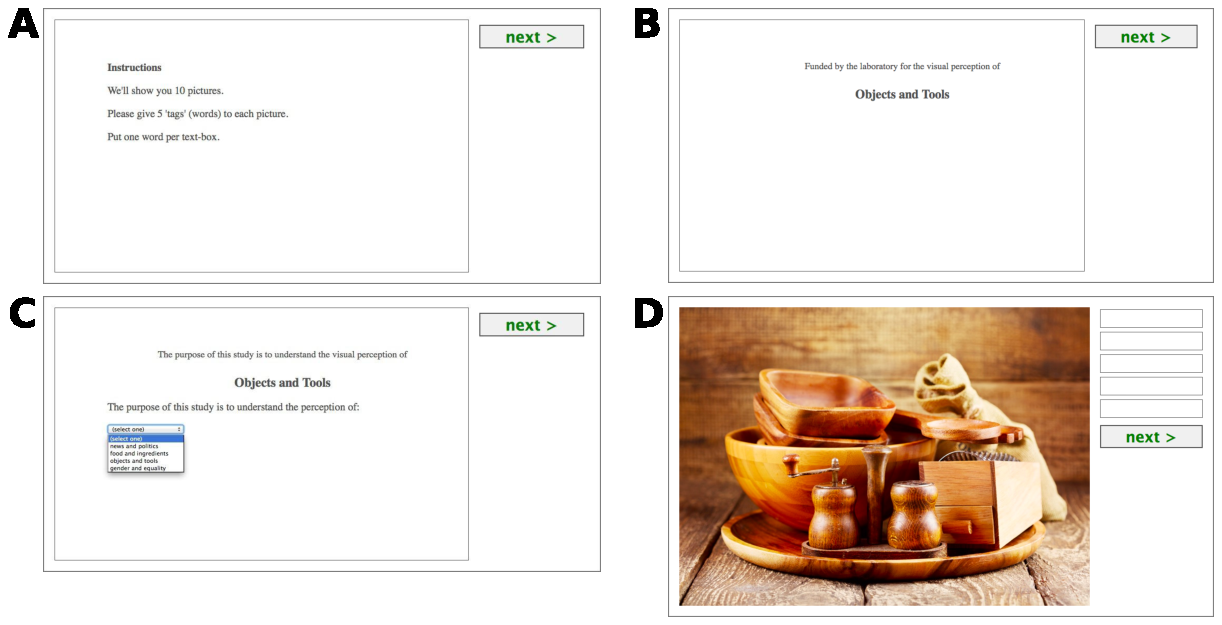
\includegraphics[scale=0.7]{figs/tasks.pdf}
	\caption{Examples of slides used for the image labeling tasks. A) instructions shown to all workers; B) a framing slide; C) a slide from the initial set for treatment IMG:FOOD; D) a slide from the initial set for treatment IMG:OBJ; E) a slide from the test set shown in all treatments. The full set of slides used for all treatments is presented in the supplementary material.}
	\label{fig:task}
\end{figure}




\paragraph{The strength of inter-task effects}
The purpose of the first experiment was to compare the relative strength
of inter-task and framing effects.  In this experiment, the treatment 
\textsc{ambg} served as a base-case.  The other treatments differed from
\textsc{ambg} either in terms of the initial image set, or by the addition of a
framing prime.  

The test images in this experiment 1 consisted of meals having
a strong, specific cultural connection (Fig. \ref{fig:task} shows an example).
The \textsc{ambg} treatment had an initial set which also consisted of meals,
but without more muted cultural overtones.  The initial images for treatment 
\textsc{img:cult} featured iconic cultural scenes (devoid of food) while 
those for treatment \textsc{img:ingr} consisted of isolated ingredients.
Treatments \textsc{frm:cult} and \textsc{frm:ingr} had the same initail images
as \textsc{ambg}, but had respectively a framing prime indicating that the
tasks were funded by a foundation for ``cultural recognition'' and
``nutritional awareness''.

We tested for inter-task effects by evaluating the performance of a Naive 
Bayes classifier when distinguishing the work-products from 
\textsc{img:cult} and \textsc{img:ingr}, and, separately, when distinguishing
those from \textsc{frm:cult} and \textsc{frm:ingr},
using only the labels that workers from these treatments
attributed to the test set of images.

can perform better than the actual difference in priming, so the performance 
of Naive Bayes classifier provides a lower bound on priming difference. We 
used leave-one-out validation to estimate the classifier per- formance. We 
tested for framing effects in a similar way, by training a Naive Bayes 
classifier to classify work-products among \textsc{frm:food} and 
\textsc{frm:obj}.

Overall, the first image in the test set showed the strongest signal for 
priming effects. Fig. 3 shows the empirical lower bound for difference in 
priming due to inter-task effects and framing based on the classifier 
performance when using labels from the first test image. Statistically 
significant levels of priming were detected for both modalities, but the 
inter-task effects were stronger (hypothesis test). This suggests that strong 
bias can result solely from the sequence of tasks performed by a worker, even 
when those tasks are of the same type.

In contrast, the classifier never performed significantly better than chance 
when distinguish- ing treatments that differed only in framing. Thus, framing 
effects were rather weak. In fact, framing effects were generally weak in our 
results, so we omit treatments involving framing from the remainder of our 
presentation to save space. We encourage the interested reader to look at the 
results for these treatments in the supplementary material.

%The first two treatments, IMG:OBJ and IMG:FOOD, tested inter-task effects. 
%Workers in these treatments labelled ten images. In the IMG:OBJ treatment, the 
%\textit{initial set} of five images labeled by workers contained objects such 
%as utensils, kitchenware, and table-settings, but no food items. In the 
%\textsc{img:food}, the initial set contained centered close-ups of meals, 
%without
%any surrounding objects (except sometimes the dish supporting the food). No 
%interruption or distinction made between the initial and test sets from the 
%view of the workers. To study the positional dependance of inter-task effects,
%these treatments were subdivided, and workers were shown one of five 
%permutations. There are of course 5! = 120 permutations of five images, but 
%investigating all permutations was too expensive, and probably redundant, so 
%we chose 5 permutations that ensure each image occupies each position within 
%the test set. We discuss the benefits and drawbacks of this choice in the 
%supplementary material.
%
%Workers in the treatments \textsc{frm:food} and \textsc{frm:obj} were shown a 
%framing slide, which bore a message reading: ``Funded by the laboratory for 
%the visual perception of \{Food and Ingredients $\vert$ Objects and Tools\}''. 
%After the framing slide, workers in these treatments proceeded directly to 
%the test set (and so labeled only 5 images).
\paragraph{Inter-task effects and the orientation of focus.}
Since the initial images were chosen to emphasize either food (ingredients 
set) or culture (cultural set), we looked for effects on the number of 
culture- and food-oriented labels that workers attributed to the test image 
set.

To this end, we constructed an ontology from the labels attributed to the test 
images. In the ontology, edges point from more general labels to more 
specific ones. For example, the ontology contains the path \texttt{food} $\to$ 
\texttt{ingredients} $\to$ \texttt{vegetables} $\to$ \texttt{tomato}.

Since food is a central feature of culture, our ontology contains many labels 
that have both food and culture in their ancestry. Nevertheless, there were 
many food-oriented labels, such as bread, which lacked specific cultural 
connections, as well as non-food, culture- orientedlabels,suchasrussian dolls.

When we tallied labels attributed to the first image of the test set, we found 
that workers from CULTimg produced significantly more culture-oriented labels 
and less food-oriented ones than those from AMBG (see Fig. 2A). The inter-task 
effect was so strong that the proportion of food- and culture-oriented labels 
in CULTimg was essentially the reverse of that in AMBG. However, the 
composition of labels attributed by INGRimg was not significantly different 
from those attributed by AMBG. This shows that inter-task effects can 
profoundly alter workers' focus. Again, we will argue later that the ambiguous 
and ingredients image sets are, in fact, quite similar.

\paragraph{Inter-task effects and specificity.}
Using the ontology described in the previous section, we can compare the 
specificity of two labels $\ell_1$ and $\ell_2$. We say that $\ell_2$ is more specific 
than $\ell_1$ if there is a directed path from $\ell_1$ to $\ell_2$. If there is no 
directed path between labels, we say they are \textit{non-comparable}. For 
example, \texttt{tomato} was more specific than \texttt{food}, while 
\texttt{statue} and \texttt{food} were non-comparable.

We can then define the relative specificity of two workers with respect to 
test-image $i$ as $s_i(u, v)$:
$$
	s_i(u,v) = \sum_{\ell \in u(i)} \sum_{\ell \in v(i)} 
	\left( \mathbf{1}_{[\ell > m]} - \mathbf{1}_{[m>\ell]} \right),
$$
where $u(i)$ denotes the set of labels attributed by worker $u$ to image $i$, 
and $\mathbf{1}_{[l>m]}$ evaluates to 1 if $\ell$ is more specific than $m$, 
and 0 otherwise. We then define the relative specificity of two treatments, 
$U$ and $V$, relative to the $i$th image, denoted $S_i(U,V)$, to be the mean 
relative specificity of two uniformly drawn workers:
$$
	\hat{S}_i(U,V) = \frac{1}{|U \times V|} \sum_{u \in U} \sum_{v in V}
		s_i(u,v).
$$
Looking at labels attributed to the first test image, we found that workers 
from \textsc{ambg} were more specific than workers from either 
$\textsc{CULT}_{img}$ or $\textsc{ingr}_{img}$.  When we compare CULTimg to 
INGRimg, we found that workers from INGRimg were more specific. This shows 
that inter-task effects do substantially influence the specificity of labels 
that workers provide. When we discuss image similarity, below, we will explore 
a possible mechanism for this effect.

\paragraph{The role of task position in inter-task effects.}
It would stand to reason that, as workers proceed through the test images, 
priming from the initial images would be ``washed out'', diminishing the 
observed
inter-task effects. Looking at the classifier performance, 
$\hat{\theta}_\mathrm{NB}$, with respect to the treatments AMBG and CULTimg, 
we find that performance does drop off dramatically after just the first image 
(see Fig. 3A). This suggests that inter-task effects primarily arise between 
consecutive tasks, but that a residual effect can persist for at least five 
tasks (we note, however that although the classifier performance seemed better 
than chance for the fourth test image, this cannot be asserted with 95\% 
confidence).

Next we observed how inter-task effects on label composition (i.e. food- vs 
culture-oriented labels) evolve as workers proceed through test images. We 
define the excess cultural orientation as the number of culture-oriented 
labels minus the number of food oriented ones. To meaning- fully compare the 
excess cultural orientation between test images, we must, however, account 
for the fact that some images inherently carry more cultural content than 
others. In keeping with our notion of priming difference, we calculate the 
excess cultural content for both CULTimg and

AMBG, and take their difference to be the relative excess cultural content, 
$\Delta_{cult}$. Formally,

		*** Formula for delta cult\ldots

where $N^(i)_{w,cult}$ stands for the number of culture-oriented labels 
attributed by worker w to image i, while $N^(i)_{w,food}$ similarly counts
food-oriented labels, and $N$ is the total number of labels in a treatment.

We found $\Delta_{cult}$ was largest for the first test image, but dropped off 
rapidly, 
remaining positive but not to a statistically significant extent (see Fig. 3B).
This is similar to the behavior of $\hat{\theta}_\mathrm{NB}$, however, 
because the statistical significance of $\Delta_{cult}$ dropped more quickly, 
$\hat{\theta}_\mathrm{NB}$ appears to be a more sensitive measure of 
inter-task effects.

\paragraph{Leveraging inter-task effects for detailed responses.}
\begin{table}
\centering
\begin{tabular}{ l  s s s s}

\toprule    
Image set   
& \multicolumn{1}{c}{Ambig.} 
& \multicolumn{1}{c}{Cultural} 
& \multicolumn{1}{c}{Ingr.}
& \multicolumn{1}{c}{Test} \\
  
\midrule

Ambiguous  & 1 & 0.0418 & 0.142 & 0.167 \\

Cultural  & 0.0418  & 1 & 0.0347 & 0.0561 \\

Ingredients  & 0.142  & 0.0347 & 1 & 0.110 \\

Test & 0.167  & 0.0561 & 0.110 & 1
\\
\bottomrule

\end{tabular}
\caption{\footnotesize{
Pairwise similarities of each image set based on the labels attributed to them (see \textbf{Eq. 4}).
}}
\label{table:2}
\end{table}

To continue with the analysis, we seek a measure of image similarity. The 
characterization of image content is a deeply complex issue that has been 
approached by many disciplines \cite{panofsky1939studies,shatford1986analyzing,Tversky1977327,Jaimes20002}. \textit{Perceptual similarity} is a 
particularly recalcitrant concept.

However, in the present study, we are more interested how similar two sets of 
images are, with respect to the labeling task, which is much simpler to 
operationalize than general percep- tual similarity. Here, we measure image 
similarity by looking at the fraction of labels that they share. Formally, to 
measure the similarity between two sets of images, X and Y , we compute the 
Jacquard index between the sets of labels attributed to them:
$$
	\mathrm{Sim}(X,Y) = \frac{L(X) \cap L(Y)}{L(X) \cup L(Y)}
$$
where $L(X)$ denotes the set of labels attributed to $X$.

The pairwise similarities of the image sets are presented in Table 2. First, 
observe that the ambiguous and ingredients sets are much more similar to each 
other than either is to the culture set. Recalling the data presented in 
Fig. 1, this helps explain why two treatments could not be distinguished on 
the basis of having differing initial sets corresponding to ambiguous and 
cultural. This also explains why AMBG and CULTimg had similar label 
compositions in Fig. 2A.

Next we draw attention to the similarity between the initial sets and the test 
set. The am- biguous set is the most similar to the test set, followed by the 
ingredients set, with the cultural set being most different. Observe that these
levels of similarity mirror the label specificity for the corresponding 
treatments (c.f. Fig. 2B).

This suggests that labeling a series of images that are similar to one another 
might encourage workers to use more specific terminology. Such a phenomenon 
would be consistent with the psychological mechanism known as 
\textit{negative priming}.
Negative priming occurs when a person becomes desensitized to non-salient 
stimuli to which she is repeatedly exposed. Consider that workers who 
initially labeled the ambiguous image set had already seen five images 
showing prepared meals once they labeled the first test image. At that point, 
a worker might not regard the generic labels \texttt{food} or \texttt{meal} to 
be salient, and opt instead for \texttt{bread}, or \texttt{pasta}.
 
We are suggesting that, although workers are not instructed to compare images 
in any way, prior tasks nevertheless create a frame of reference relative to 
which later tasks are judged. This in turn influences the perception of 
salience. Thus, in a series of subjective characterization tasks that have 
very similar content, workers' focus will tend to be directed away from 
generic, shared attributes, towards those attributes that are specific and 
distinguishing.

\paragraph{Conclusions.}
Our results show that inter-task effects can have a strong influence on how 
workers label images. In particular, we observed that prior tasks influence 
the specificity and content of labels. Surprisingly, framing a task by 
indicating a semantically-loaded funder had much milder effects on worker 
outputs, generally below the statistical power of our tests.

We therefore caution those designing studies using human computation: even if 
the requester has eliminated surrounding influences to every practical extent, 
\textit{the greatest source of bias might lurk in the tasks themselves}. Due 
consideration should be given to how tasks are bundled together. While our 
measurements of $\hat{\theta}_\mathrm{NB}$ indicated that inter-task effects 
persisted even to the fifth test image, the most severe effects arise between 
consecutive tasks.

Our proposed priming definition yields general purpose measure of priming 
effects. We used three approaches to detect priming effects: 1) using a Naive 
Bayes classifier to measure $\hat{\theta}_\mathrm{NB}$, 2) tallying the 
number of culture- and food-oriented labels, and 3) comparing the relative
specificity of labels based on an ontology. Of the three, $\theta_\mathrm{NB}$ 
was the most sensitive.

In one sense, this is not surprising because the Naive Bayes classifier takes 
into account the frequency of occurrence of all labels encountered during 
training. But it is remarkable that the method which incorporates neither 
prior knowledge about the image contents nor label semantics, outperforms 
those that do. This is a powerful feature because, given the outputs from two 
sets of workers, one can test whether they have been differently primed 
without knowing how that priming might manifest.

Our algorithmic definition of priming is phrased in terms of worker outputs 
rather than psychological phenomena. This provides a connection between the 
priming effects and their potential to impact decisions made on the basis of 
worker outputs. In the case of a 1-bit binary decision, $\theta$ describes the 
worst-case bias introduced by failing to control for priming effects.

Batching similar tasks together appears to yield higher more specific HPU 
outputs. Our proposed connection between similarity and specificity during 
image-labeling might be used to tune the specificity of labels. For example, 
If one seeks very nuanced labeling, our results suggest that the images 
should first be sorted into batches based on their similarity. This could be 
accomplished by beginning with a first, coarse labeling of unsorted images, 
followed by bundling based on the similarity of coarse labels. Then, bundles 
of similar images could be served for a second round of finer labeling. The 
sorting and re-labeling could in principle be repeated.

Such a workflow involves serial processing, which points to an interesting 
possible differ- ence difference between HPUs and CPUs. In general, whenever 
an aspect of a problem can be parallelized when employing CPUs, one gains 
efficiency. But here, because of HPU hysteresis, one might gain precision by 
using HPUs with a more serialized algorithm. Further testing is needed to 
determine the gain in precision from this approach.


\bibliography{newbib}
\bibliographystyle{Science}



\end{document}




















